
\begin{frame} \frametitle{Wavelet transforms for EXAFS analysis}


... and wavelets may be most useful for such structures with overlapping shells:



\begin{columns}
  \begin{column}[T]{75mm}
    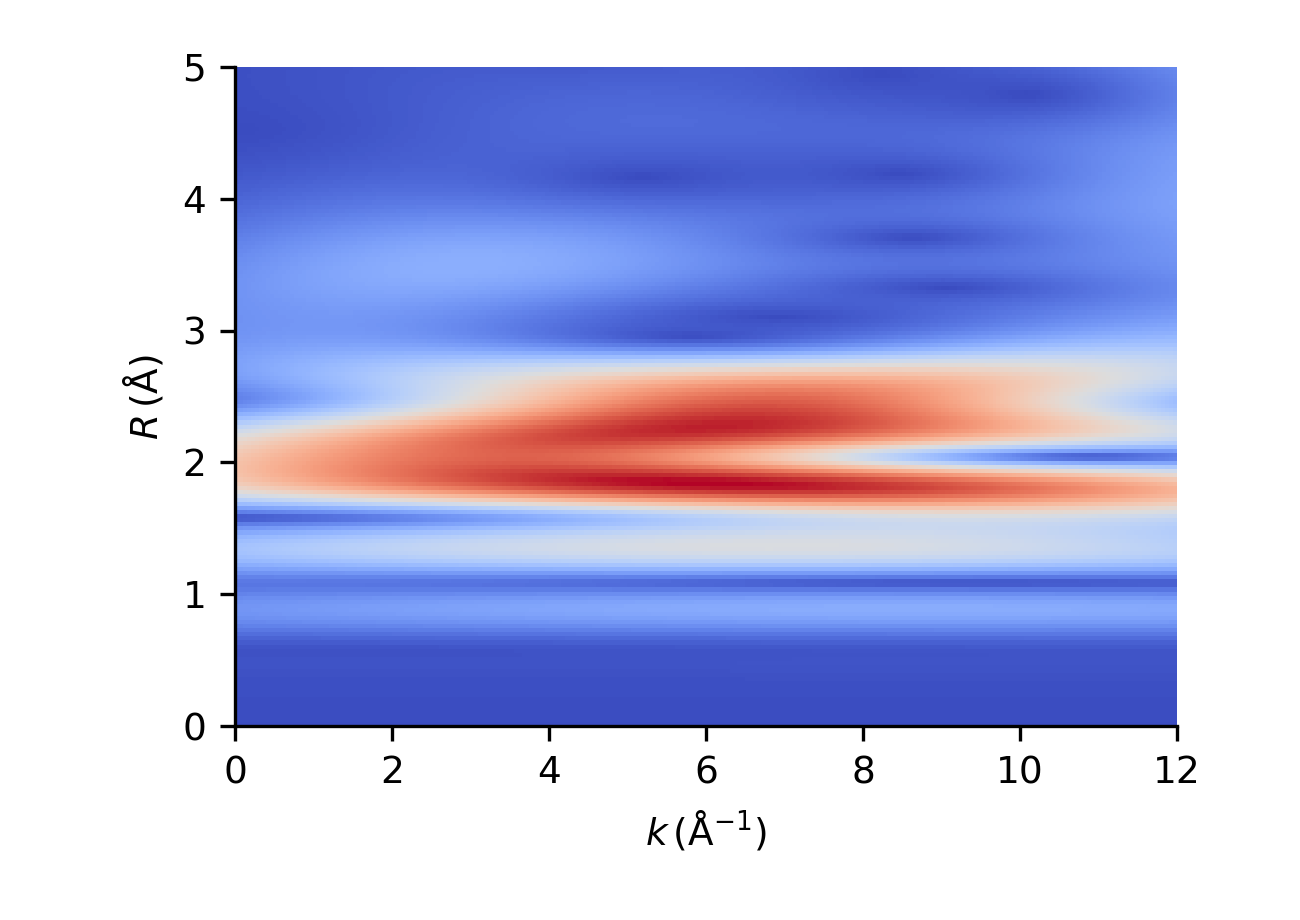
\includegraphics[width=75mm]{figs/wavelets/mnco3cp_data_mag}
  \end{column}
  \begin{column}[T]{25mm}

    \vspace{5mm}

  \hspace{-7mm}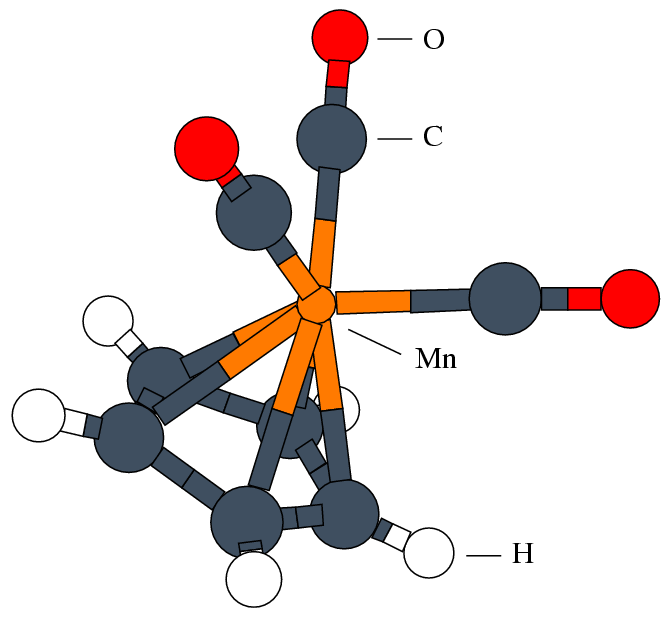
\includegraphics[width=27mm]{figs/wavelets/mnco3}

\end{column}
\end{columns}

\vmm

\begin{cenpage}{90mm}
This spectra has strong mixing of single- and multiple-scattering
paths, even in the first shell.

\vmm

The diagonals of intensity show complicated interferences, and may
be a useful clue that even the first shell is not well-isolated.


\end{cenpage}

\end{frame}
